\section{Λευκός Θόρυβος} \label{sec:white_noise}

Στην επεξεργασία σημάτων ο λευκός θόρυβος, είναι ένα τυχαίο σήμα, που έχει σταθερή ένταση σε όλες τις συχνότητες, δηλαδή σταθερή πυκνότητα φάσματος ισχύος \cite{Carter2009}. Ο όρος χρησιμοποιείται σε διάφορους τομείς, όπως η φυσική, οι τηλεπικοινωνίες και η ακουστική. Στον διακριτό χρόνο, ο λευκός θόρυβος είναι ένα διακριτό σήμα, του οποίου τα δείγματα αντιμετωπίζονται ως μία σειρά ασυσχέτιστων τυχαίων μεταβλητών, με μέση τιμή μηδέν, και πεπερασμένη απόκλιση. Εφόσον ο λευκός θόρυβος ακολουθεί την κατανομή που περιγράφεται στην εξίσωση \ref{eq 4}, αποκαλείται Additive White Gaussian Noise (AWGN). Αξίζει να σημειωθεί πως ο λευκός θόρυβος είναι μια καθαρά θεωρητική κατασκευή, από την άποψη ότι δεν υφίστανται σήματα με άπειρο εύρος ζώνης. Τυπικά ένα σήμα λευκού θορύβου έχει τη μορφή που φαίνεται στο Σχήμα \ref{fig:typical_white_noise}

\begin{CEquation}
    Z_n \sim N(0,W) \label{eq 4}
\end{CEquation}

\begin{figure}[h]
  \centering
  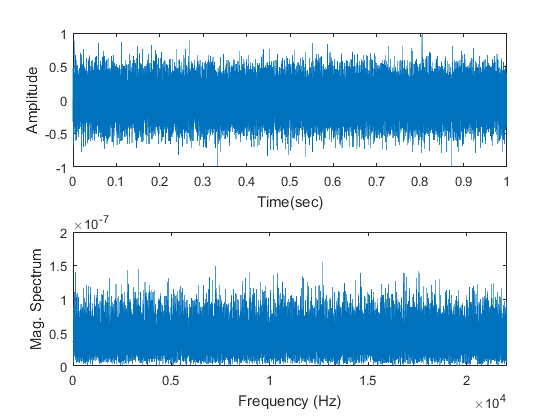
\includegraphics[width=\textwidth, height=8cm]{images/typical_white_noise.png}
  \caption{Τυπική μορφή σήματος λευκού θορύβου, στον χρόνο (Πάνω) και στη συχνότητα (Κάτω)}
  \label{fig:typical_white_noise}
\end{figure}